
%(BEGIN_QUESTION)
% Copyright 2014, Tony R. Kuphaldt, released under the Creative Commons Attribution License (v 1.0)
% This means you may do almost anything with this work of mine, so long as you give me proper credit

Imagine you are using a digital voltmeter to measure voltages between pairs of points in a circuit, following the sequence of steps shown in the following diagrams:

$$\includegraphics[width=15.5cm]{i01158x01.eps}$$

How much voltage would be registered by the voltmeter in each of the steps?  Be sure to include the sign of the DC voltage measured (note the coloring of the voltmeter leads, with the red lead always on the first point denoted in the subscript: $V_{BA}$ = red lead on ``B'' and black lead on ``A''):

\begin{itemize}
\item{} $V_{BA} = $
\item{} $V_{DB} = $
\item{} $V_{FD} = $
\item{} $V_{AF} = $
\end{itemize}

What is the algebraic sum of these voltages?

\underbar{file i01158}
%(END_QUESTION)





%(BEGIN_ANSWER)

\begin{itemize}
\item{} $V_{BA} = +10.8$ volts
\item{} $V_{DB} = +25.2$ volts
\item{} $V_{FD} = -12.0$ volts
\item{} $V_{AF} = -24.0$ volts
\end{itemize}

%(END_ANSWER)





%(BEGIN_NOTES)

Ask your students this question: ``Will the algebraic sum of voltage measurements ever be other than zero in a loop?''  Ask them to explain {\it why} this is, as best they can.

%INDEX% Electronics review: series-parallel circuits

%(END_NOTES)


